\section{Arquitectura del motor de inteligencia artificial}
\label{sec:motor-ia}

El Marco Teórico presentó el enfoque híbrido en tres capas sobre el que se organiza el motor de recomendaciones (Sección~\ref{sec:sistemas-recomendacion}): una capa predictiva, una capa de reglas de negocio por rubro y una capa de aprendizaje por refuerzo para la priorización, a las que se suma un modelo de lenguaje que solo redacta. Esta sección describe cómo el prototipo implementa cada capa: el flujo de datos que las conecta, los algoritmos con sus parámetros, las seis reglas con sus umbrales por rubro, el calendario de fechas clave, la regla de actualización del bandit y el criterio con el que se ordenan las recomendaciones. Cierra con la forma en que se evalúa el motor, cuyos resultados se presentan en la Sección~\ref{sec:evaluacion-modelos}.

\subsection{Flujo de datos entre las capas}
\label{sec:motor-flujo}

El motor se ejecuta en el proceso de tareas en segundo plano (\emph{worker}), separado de la API, y se encadena a la sincronización de los datos de cada tienda. La Figura~\ref{fig:motor-capas} resume el recorrido. Cada sincronización, ya sea la incremental, que se repite cada seis horas, o la que disparan los webhooks de la plataforma, deja los datos en el modelo canónico del sistema y encola el recálculo del pronóstico de demanda y de la segmentación de clientes (capa predictiva). Al terminar, se encola la ejecución del motor, que resuelve el rubro de la tienda, aplica las seis reglas sobre las predicciones (capa de reglas) y asigna a cada recomendación el puntaje de su tipo según el bandit (capa de priorización). Antes de guardarla, el modelo de lenguaje redacta su mensaje (capa de explicación). Cuando el comerciante abre el panel, la API ordena las recomendaciones activas con una muestra de Thompson Sampling del día.

\begin{figure}[!htbp]
\centering
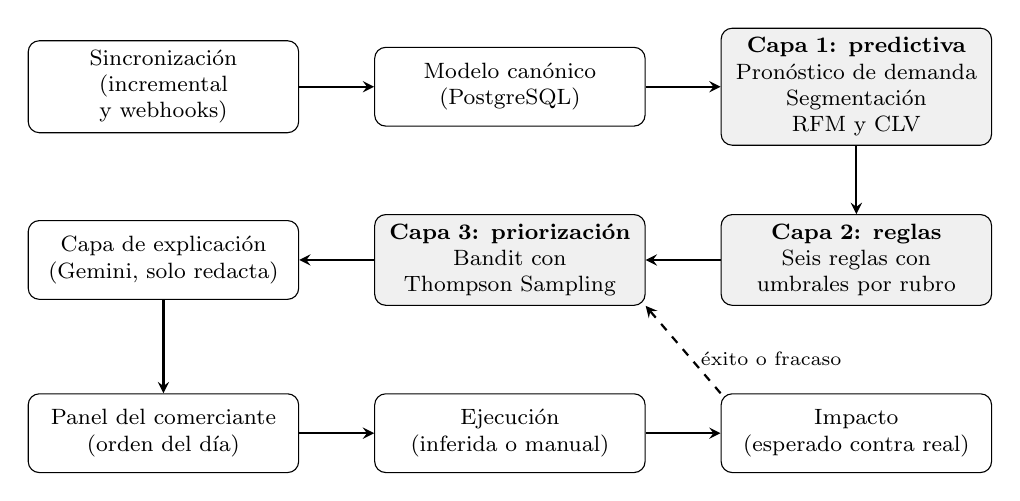
\begin{tikzpicture}[
    caja/.style={draw, rounded corners, align=center, font=\footnotesize, minimum height=1cm, text width=3.2cm},
    capa/.style={caja, fill=gray!12},
    flecha/.style={-stealth, thick}]
  \node[caja] (sync) at (0,0) {Sincronización\\(incremental y webhooks)};
  \node[caja] (canon) at (4.4,0) {Modelo canónico\\(PostgreSQL)};
  \node[capa] (pred) at (8.8,0) {\textbf{Capa 1: predictiva}\\Pronóstico de demanda\\Segmentación RFM y CLV};
  \node[capa] (reglas) at (8.8,-2.2) {\textbf{Capa 2: reglas}\\Seis reglas con\\umbrales por rubro};
  \node[capa] (bandit) at (4.4,-2.2) {\textbf{Capa 3: priorización}\\Bandit con\\Thompson Sampling};
  \node[caja] (llm) at (0,-2.2) {Capa de explicación\\(Gemini, solo redacta)};
  \node[caja] (panel) at (0,-4.4) {Panel del comerciante\\(orden del día)};
  \node[caja] (ejec) at (4.4,-4.4) {Ejecución\\(inferida o manual)};
  \node[caja] (impacto) at (8.8,-4.4) {Impacto\\(esperado contra real)};
  \draw[flecha] (sync) -- (canon);
  \draw[flecha] (canon) -- (pred);
  \draw[flecha] (pred) -- (reglas);
  \draw[flecha] (reglas) -- (bandit);
  \draw[flecha] (bandit) -- (llm);
  \draw[flecha] (llm) -- (panel);
  \draw[flecha] (panel) -- (ejec);
  \draw[flecha] (ejec) -- (impacto);
  \draw[flecha, dashed] (impacto.north west) -- node[font=\scriptsize, right, pos=0.4] {éxito o fracaso} (bandit.south east);
\end{tikzpicture}
\caption{Capas del motor de recomendaciones y flujo de datos entre ellas.}
\label{fig:motor-capas}

\smallskip
\noindent\textit{Fuente: elaboración propia.}
\end{figure}

El ciclo se cierra con dos tareas adicionales. Después de cada sincronización incremental, la inferencia de ejecuciones compara las fotos de stock y precio de las variantes con lo que proponía cada recomendación activa. Una vez por día, a las 5 de la mañana (hora de Argentina), la evaluación de impacto compara el resultado real de las recomendaciones cuya ventana terminó con el esperado que se fijó al generarlas, registra cada resultado como éxito o fracaso en el bandit y recalcula las distribuciones previas de cada rubro.

\subsection{Capa predictiva}
\label{sec:motor-predictiva}

La capa predictiva produce dos insumos para las reglas: el pronóstico diario de unidades de cada variante y la segmentación de los clientes de la tienda.

\paragraph{Pronóstico de demanda.} Para cada variante se construye la serie de unidades vendidas por día en órdenes pagadas, con hasta 180 días de historia y los días cortados en hora de Argentina. La serie comienza en la primera venta, porque los ceros previos a la publicación del producto no son demanda. Sobre esa historia se elige el modelo según tres casos:

\begin{itemize}
    \item con menos de 14 días de historia, suavizado exponencial simple;
    \item si más del 60\% de los días no registra ventas (demanda intermitente), promedio móvil de los últimos 28 días, marcado como pronóstico de baja confianza;
    \item en los demás casos, Holt-Winters aditivo con estacionalidad semanal ($m = 7$).
\end{itemize}

Los parámetros de suavizado se eligen por búsqueda en grilla, minimizando el error cuadrático de los pronósticos a un paso: $\alpha$ y $\gamma$ toman los valores 0,05; 0,1; 0,2; 0,3; 0,5; 0,7 y 0,9, y $\beta$, los valores 0,01; 0,05; 0,1 y 0,2. La tendencia se limita a valores bajos para que no se dispare al extrapolar dos o tres semanas. El horizonte del pronóstico es el mayor entre 14 días, el umbral de alerta de quiebre y la ventana de impacto del rubro, y la ventana completa de una fecha clave recomendada con su anticipación; en la práctica, 17 días para gastronomía e indumentaria y 21 para electrónica. Antes de pronosticar, el modelo se valida reservando los últimos 14 días de la serie: se ajusta con el resto y su WAPE se compara con el de dos referencias, un pronóstico plano igual al promedio de los últimos 28 días y uno semanal ingenuo que repite la última semana observada.

El efecto de las fechas clave se estima con la historia de cada tienda: para cada ocurrencia pasada de una fecha, se divide la venta total de la tienda en la ventana de la fecha por la venta esperada sin ella, calculada como el promedio del mismo día de la semana en los 28 días previos, excluidos los días de otras fechas clave. La estimación requiere al menos 14 días de referencia válidos y nunca baja de 1. Si no se puede estimar, se usa el factor típico del rubro (Tabla~\ref{tab:motor-fechas}).

\paragraph{Segmentación de clientes.} A partir de las órdenes pagadas se calculan la recencia, la frecuencia y el monto de cada cliente. Las tres variables se transforman en $[R,\ \log(1+F),\ \log(1+M)]$, donde el logaritmo reduce el peso de los pocos clientes que concentran muchas compras, y se normalizan a puntajes $z$. Sobre esos puntos se ejecuta k-means con inicialización k-means++ y semilla fija (42), para que el resultado sea reproducible, con $k \in \{3, 4, 5\}$; se conserva el valor de $k$ con mayor coeficiente de silueta. Cada grupo se etiqueta según su centroide:

\begin{itemize}
    \item \emph{campeones}: el de mayor puntaje $-R + F + M$;
    \item \emph{perdidos}: entre los demás, el de mayor recencia;
    \item \emph{en riesgo}: los grupos cuya recencia media supera el doble de su intervalo habitual entre compras;
    \item \emph{leales} u \emph{ocasionales}: los restantes, según su frecuencia esté en la media o por encima, o por debajo de ella.
\end{itemize}

El umbral de inactividad de la tienda es el máximo entre el piso del rubro y la mediana de días entre compras de sus clientes multiplicada por el factor del rubro (Tabla~\ref{tab:motor-umbrales}). El CLV de cada cliente se calcula como el ticket promedio por las compras anuales, con una antigüedad mínima de 30 días para no anualizar de más, y por la vida esperada en años, igual a la inversa de la tasa de abandono de la tienda con un tope de cinco años. Por último, para cada segmento se mide la tasa histórica de retorno: en cortes semanales, la proporción de clientes inactivos que volvieron a comprar dentro de la ventana de impacto del rubro. Esa tasa es el esperado contra el que se mide una recomendación de retención.

\subsection{Capa de reglas por rubro}
\label{sec:motor-reglas}

\paragraph{Resolución del rubro.} Las reglas usan los parámetros del rubro efectivo de la tienda. Si el rubro declarado es uno de los tres soportados, se usa ese. En otro caso, por ejemplo en las tiendas de Tiendanube que ingresan con tipo \emph{general}, se infiere de los nombres de las categorías y los productos mediante listas de palabras clave por rubro: la inferencia es concluyente si al menos tres nombres coinciden con alguna lista y un rubro reúne el 60\% de las coincidencias. Si no lo es, se usan parámetros genéricos, iguales a los de indumentaria, y la recomendación se marca para que la interfaz lo advierta.

\paragraph{Reglas.} El motor aplica seis reglas, resumidas en la Tabla~\ref{tab:motor-reglas}. Cada una decide si corresponde recomendar, con qué nivel de prioridad (urgente, atención u oportunidad) y con qué puntaje propio, de 0 a 100, que ordena las recomendaciones de un mismo tipo. Al generar la recomendación, la regla guarda también el resultado esperado contra el que luego se medirá su impacto. Las reglas no repiten una recomendación que ya está activa para el mismo objetivo.

\begin{table}[!htbp]
\centering
\caption{Reglas del motor: condición, prioridad, puntaje y esperado para medir el impacto}
\label{tab:motor-reglas}
\renewcommand{\arraystretch}{1.3}
\footnotesize
\setlength{\tabcolsep}{3pt}
\begin{tabular}{|>{\raggedright\arraybackslash}m{2.2cm}|>{\raggedright\arraybackslash}m{4.1cm}|>{\raggedright\arraybackslash}m{2.6cm}|>{\raggedright\arraybackslash}m{1.9cm}|>{\raggedright\arraybackslash}m{2.4cm}|}
\hline
\textbf{Regla} & \textbf{Condición y variables} & \textbf{Prioridad} & \textbf{Puntaje} & \textbf{Esperado} \\
\hline
Quiebre de stock (RF-08, HU-01) & Días hasta agotar el stock $d$, acumulando la demanda pronosticada día por día; recomienda si $d \le$ umbral de alerta. Solo variantes con gestión de stock & Urgente si $d \le$ umbral urgente; si no, atención & $100\,(1 - d/\text{alerta})$ & Unidades pronosticadas en la ventana de impacto \\
\hline
Preparación anticipada (HU-02) & Día pico entre 2 y 7 días adelante con pronóstico $\ge$ 130\% del promedio reciente y al menos 1 unidad; excluye pronósticos de baja confianza y, dentro de una fecha clave, los productos no destacados & Atención si el pico está a 3 días o menos; si no, oportunidad & Suba porcentual del pico & Unidades pronosticadas en la ventana de impacto \\
\hline
Fecha clave (HU-06) & Fecha del rubro entre 1 y 14 días adelante; promoción sobre los 5 productos con más unidades vendidas en los últimos 28 días; una recomendación por ocurrencia & Oportunidad & Suba esperada, $(\text{factor} - 1) \times 100$ & Pronóstico de los destacados en la ventana de la fecha, por el factor \\
\hline
Baja rotación (RF-09, HU-03) & Caída de las unidades vendidas en la última ventana del rubro frente a la anterior; recomienda si la caída $\ge$ umbral del rubro & Atención & Caída porcentual & Pronóstico de la ventana o, sin pronóstico, el ritmo reciente \\
\hline
Revisión de precio (RF-10, HU-05) & Días desde el último cambio de precio $\ge$ umbral del rubro; en tiendas en pesos, variación del dólar desde ese cambio & Oportunidad si el dólar subió más que el umbral; si no, atención & $50\,d/\text{umbral}$, más la variación del dólar & Precio anterior (ingreso por unidad) \\
\hline
Riesgo de abandono (RF-13, HU-10) & Días sin comprar mayores que el umbral de inactividad de la tienda & Urgente si el cliente es \emph{en riesgo} o \emph{campeón} con CLV en el cuartil superior; si no, atención & Percentil de CLV entre los inactivos & Tasa de retorno del segmento \\
\hline
\end{tabular}

\smallskip
\noindent\textit{Fuente: elaboración propia sobre la base del código del prototipo.}
\end{table}

\paragraph{Umbrales por rubro y constantes fijas.} Los umbrales que diferencian a los rubros se resumen en la Tabla~\ref{tab:motor-umbrales}. Se definieron a partir de las entrevistas del Anexo B y de las particularidades de cada rubro descriptas en la Sección~\ref{sec:comportamiento-consumidor}, y se configuran sin modificar las reglas. Además de estos umbrales, el motor usa constantes iguales para todos los rubros: en la preparación anticipada, un pico de al menos 30\% sobre el promedio reciente, una anticipación mínima de 48 horas, un alcance de 7 días y el nivel de atención a 3 días o menos; en las fechas clave, una anticipación de 14 días y 5 productos destacados; en el abandono, el cuartil superior de CLV para la prioridad urgente; y en la inferencia de ejecuciones, una suba del stock de al menos 20\% del stock de base (como mínimo una unidad) para una reposición, un cambio de precio de al menos 1\% para una revisión de precio y una baja de al menos 5\% para una promoción por baja rotación.

\begin{table}[!htbp]
\centering
\caption{Umbrales de las reglas por rubro}
\label{tab:motor-umbrales}
\renewcommand{\arraystretch}{1.3}
\footnotesize
\setlength{\tabcolsep}{4pt}
\begin{tabular}{|>{\raggedright\arraybackslash}m{6.4cm}|r|r|r|}
\hline
\textbf{Parámetro} & \textbf{Gastronomía} & \textbf{Indumentaria} & \textbf{Electrónica} \\
\hline
Días hasta el quiebre para alertar & 3 & 14 & 21 \\
\hline
Días hasta el quiebre para prioridad urgente & 1 & 5 & 7 \\
\hline
Ventana de comparación de rotación (días) & 7 & 15 & 30 \\
\hline
Caída de rotación para alertar & 25\% & 30\% & 30\% \\
\hline
Días sin actualizar el precio & 30 & 45 & 15 \\
\hline
Variación del dólar para oportunidad & 15\% & 10\% & 5\% \\
\hline
Multiplicador del ciclo de recompra & 2 & 2 & 2 \\
\hline
Piso de inactividad del cliente (días) & 21 & 60 & 120 \\
\hline
Ventana de evaluación del impacto (días) & 7 & 14 & 21 \\
\hline
\end{tabular}

\smallskip
\noindent\textit{Fuente: elaboración propia sobre la base del código del prototipo.}
\end{table}

\paragraph{Umbrales dinámicos.} Dos de los umbrales que usa el motor no son fijos sino que se calculan para cada tienda. El primero es el umbral de inactividad de los clientes, que combina el piso del rubro con el ciclo de recompra observado en la propia tienda, como se describió en la Sección~\ref{sec:motor-predictiva}. El segundo es el horizonte del quiebre de stock: la alerta no compara el stock con un consumo promedio fijo, sino con la demanda pronosticada para la variante, que incorpora su estacionalidad semanal y el efecto de las fechas clave.

\paragraph{Calendario de fechas clave.} La Tabla~\ref{tab:motor-fechas} presenta el calendario con el factor de suba típico de cada fecha por rubro. Un factor de 1,6, por ejemplo, indica una venta 60\% superior a la habitual durante la ventana de la fecha. Las fechas sin factor para un rubro no generan recomendaciones en él. Las fechas de los eventos de la Cámara Argentina de Comercio Electrónico, Hot Sale y CyberMonday, se cargan por año.

\begin{table}[!htbp]
\centering
\caption{Calendario de fechas clave con su factor de suba por rubro}
\label{tab:motor-fechas}
\renewcommand{\arraystretch}{1.3}
\footnotesize
\setlength{\tabcolsep}{4pt}
\begin{tabular}{|>{\raggedright\arraybackslash}m{2.8cm}|>{\raggedright\arraybackslash}m{3.6cm}|>{\raggedright\arraybackslash}m{2.4cm}|r|r|r|}
\hline
\textbf{Fecha} & \textbf{Cálculo} & \textbf{Ventana} & \textbf{Gastr.} & \textbf{Indum.} & \textbf{Electr.} \\
\hline
San Valentín & 14 de febrero & 7 días antes & 1,3 & 1,2 & 1,1 \\
\hline
Vuelta a clases & Configurada por año & 13 días antes & --- & 1,3 & 1,3 \\
\hline
Hot Sale & Configurada por año & 3 días & 1,2 & 1,6 & 1,7 \\
\hline
Día del Padre & Tercer domingo de junio & 7 días antes & 1,2 & 1,4 & 1,5 \\
\hline
Día del Amigo & 20 de julio & 3 días antes & 1,4 & --- & --- \\
\hline
Día de las Infancias & Tercer domingo de agosto & 7 días antes & --- & 1,3 & 1,4 \\
\hline
Día de la Madre & Tercer domingo de octubre & 7 días antes & 1,3 & 1,5 & 1,3 \\
\hline
CyberMonday & Configurada por año & 3 días & 1,2 & 1,6 & 1,8 \\
\hline
Black Friday & Viernes posterior al cuarto jueves de noviembre & El día & --- & 1,4 & 1,6 \\
\hline
Navidad & 25 de diciembre & 7 días antes & 1,6 & 1,5 & 1,6 \\
\hline
\end{tabular}

\smallskip
\noindent\textit{Fuente: elaboración propia sobre la base del código del prototipo.}
\end{table}

\subsection{Capa de priorización}
\label{sec:motor-bandit}

La capa de priorización implementa el bandido multibrazo descripto en la Sección~\ref{sec:aprendizaje-refuerzo}. Cada tienda tiene seis brazos, uno por tipo de recomendación, y cada brazo mantiene una distribución Beta$(\alpha, \beta)$ sobre la probabilidad de que una recomendación de ese tipo resulte exitosa en esa tienda.

\paragraph{Distribución previa.} Cuando una tienda no tiene todavía un brazo para un tipo, se crea con la distribución previa de su rubro, calculada con los resultados de todas las tiendas del mismo rubro: con $s$ éxitos y $f$ fracasos, la tasa suavizada es $p = (s + 1)/(s + f + 2)$, y la previa es Beta$(1 + 2p,\ 1 + 2(1 - p))$, que equivale siempre a cuatro observaciones. Si el rubro todavía no tiene resultados, se usa Beta$(2, 2)$, de media 0,5. Así, una tienda nueva aprovecha lo aprendido en su rubro, pero su propia evidencia pasa a dominar rápidamente.

\paragraph{Regla de actualización.} La evaluación diaria de impacto convierte cada recomendación cerrada en un resultado binario:

\begin{itemize}
    \item \emph{éxito}, si se ejecutó y su impacto medido como esperado contra real fue positivo: se suma uno a $\alpha$;
    \item \emph{fracaso}, si se ejecutó sin impacto positivo o sin dato para medirlo, o si venció sin ejecutarse: se suma uno a $\beta$.
\end{itemize}

Cada recomendación se cuenta una sola vez. Después de actualizar los brazos, se recalculan las distribuciones previas de cada rubro, agrupando cada resultado por el rubro con el que el motor generó la recomendación.

\paragraph{Orden de las recomendaciones.} El panel ordena las recomendaciones activas con tres criterios sucesivos. Primero, el nivel de prioridad que fijó la regla: las urgentes, luego las de atención y por último las oportunidades. Dentro de un mismo nivel, la muestra de Thompson Sampling del tipo de cada recomendación, de mayor a menor. Dentro de un mismo tipo, el puntaje de la regla. Las muestras se toman con un generador pseudoaleatorio cuya semilla combina la tienda y el día, de modo que el orden no cambia durante el día y una demostración puede repetirse. El nivel de prioridad tiene precedencia sobre el aprendizaje porque responde a la urgencia del caso, como un quiebre de stock inminente, que el historial de éxitos de un tipo no debe postergar. Cada recomendación guarda, además, la media posterior de su brazo multiplicada por 100 como puntaje de referencia, y el panel muestra una explicación breve de lo aprendido; por ejemplo: «En tu tienda se ejecutaron 4 recomendaciones de este tipo y 3 de 4 evaluadas tuvieron impacto positivo».

\subsection{Capa de explicación}
\label{sec:motor-explicacion}

El texto de cada recomendación lo redacta el modelo Gemini 3.5 Flash-Lite, configurable mediante una variable de entorno para poder reemplazarlo sin modificar el código si el proveedor lo discontinúa. El modelo recibe el rubro, el tipo de recomendación, su objetivo, las métricas que calculó la regla y el contexto de las capas anteriores: el pronóstico, la fecha clave, el segmento y el CLV del cliente, y la explicación de la priorización. Devuelve, con un esquema JSON definido, un mensaje breve para la tarjeta y una explicación más extensa para la pantalla de detalle. Las instrucciones le indican que use únicamente los números recibidos, sin calcular ni inventar cifras: el modelo no interviene en qué se recomienda ni en qué orden.

Antes del envío, el nombre del cliente se reemplaza por un marcador que se restituye al recibir la respuesta, de modo que ningún dato personal sale del servidor. Los textos que provienen de la tienda, como los nombres de productos, se tratan como datos no confiables frente a una posible inyección de instrucciones: se reducen a una línea de hasta 120 caracteres, sin caracteres de control, enlaces ni delimitadores, y viajan dentro de un bloque de datos separado de las instrucciones. La respuesta se valida antes de usarse: debe incluir los dos textos dentro de su largo máximo, sin enlaces y mencionando el objetivo de la recomendación. Si la validación falla, o si el servicio no responde, se utiliza un texto de respaldo generado por plantilla, y la recomendación registra cuál de las dos fuentes produjo su texto. El detalle de estas mitigaciones se desarrolla en la sección de seguridad.

\subsection{Evaluación del motor}
\label{sec:motor-evaluacion}

Cada capa se evalúa con un criterio propio. El pronóstico se evalúa con el WAPE sobre los 14 días reservados de cada variante, agregado por rubro y ponderado por el volumen vendido, y se compara con las dos referencias ingenuas: un modelo que no las mejora no aporta información sobre ellas. La segmentación se evalúa con el coeficiente de silueta del valor de $k$ elegido en cada tienda. Las reglas se evalúan, recomendación por recomendación, con el impacto medido como esperado contra real, que constituye una correlación indicativa y no una prueba de causalidad (Sección~\ref{sec:feedback-loop}). El bandit se evalúa por la evolución de las distribuciones de sus brazos a medida que se acumulan resultados. Tres comandos del sistema generan estos indicadores sobre los datos de cualquier tienda: el reporte del pronóstico, el de la segmentación y el del bandit.

Las métricas del pronóstico y de la segmentación pueden calcularse sobre datos históricos, sintéticos o reales. Las de las reglas y del bandit, en cambio, requieren que comerciantes reales ejecuten las recomendaciones y que se observe su resultado, por lo que con los datos disponibles demuestran el funcionamiento del mecanismo y no su efectividad. Los resultados de cada evaluación, y esta limitación, se presentan en la Sección~\ref{sec:evaluacion-modelos}.
